\documentclass{article}
\usepackage{graphicx} % Required for inserting images
\usepackage{tikz}
\usetikzlibrary{arrows.meta, shapes.multipart, positioning, calc}
\usepackage{graphicx} % Required for inserting images
\usepackage{tcolorbox}
\usepackage{xcolor}

\title{SDF Project-1 Report}
\author{Sriraj Vasanta\\CS24BTECH11066}
\date{May 2025}

\begin{document}

\maketitle
\section{Introduction}
The CS1023 course project involved developing a custom arbitrary-precision arithmetic library in Java, designed to deepen understanding of numerical computation beyond Java's built-in BigInteger and BigDecimal classes.\newline
This library enables precise manipulation of integers exceeding Integer.MAX\_VALUE ($2^{32}-1$) and floating-point numbers with up to 30 decimal places. Unlike standard libraries, it prioritizes pedagogical value by requiring ground-up implementation of core algorithms and data structures for arbitrary-precision arithmetic
\section{Design}
\subsection{Overview}
\begin{itemize}
    \item \textbf{Sign handling:} Sign has been handled separately by removing it at the start and then adding the proper sign at the end.
    \item \textbf{Input validation:} This involves checking if alphabets, more than two decimal points, or more that two minus signs are present in the input.
    \item \textbf{Exception handling:} The use of argprse library in MyInfArith.py handles most of the errors caused by invalid inputs. The other errors are handled manually.
    \item \textbf{Optimisation:} AInteger.java methods were invoked to solve the operations in AFloat.java. Division was also slightly optimized by comparing the string length.
\end{itemize}
\subsection{Files description}
\begin{itemize}
    \item \textbf{AInteger.java} - Handles operations between arbitrarily large integers.
    \item \textbf{AFloat.java} - Handles operation between floating-points with arbitrary precision.
    \item \textbf{MyInfArith.py} - Imports both the classes to simpler use.
\end{itemize}
\section{File Structure}
\begin{verbatim}
    Actual/
    |-- arbitraryarithmetic/
    |   |--> AInteger.java
    |   |--> AInteger.class
    |   |--> AFloat.java
    |   |--> AFloat.class
    |--reports/
    |   |--> Report.pdf
    |   |--> Report.tex
    |-- .gitignore
    |-- Dockerfile
    |-- MyInfArith.java
    |-- MyInfArith.py
    |-- README.md
    |-- build.xml
\end{verbatim}
\section{Implementation Logic}
\subsection{AInteger.java}
\subsubsection{Addition}
\begin{itemize}
    \item For numbers of the same sign, traditional digit-by-digit addition was implemented. Carries were properly managed and propagated to the subsequent digits.
    \item For numbers of the opposite sign the subtraction method of the class was used.\footnote{\label{1}This approach leverages Java's flexibility, which allows a method to be called before it is defined, provided it exists somewhere in the same file.}
    \item The final sign was determined and added after the numerical operation. For example, the sum of two negative numbers was computed as the sum of their absolute values, with a negative sign appended to the result.
\end{itemize}
\subsubsection{Subtraction}
\begin{itemize}
    \item For numbers of the same sign typical digit-by-digit subtraction was implemented (properly storing the carry and using it for the next digits).
    \item For numbers of the opposite sign addition method was used.\textsuperscript{\ref{1}}
    \item As with addition, the final sign was determined at the end of the operation based on the original operands.
\end{itemize}
\subsubsection{Multiplication}
\begin{itemize}
    \item The absolute values of the numbers were for the core multiplication logic. The sign of the final result was determined and stored separately (using a boolean flag), and applied after the multiplication.
    \item Traditional long multiplication was implemented: each digit of the second number was multiplied with the first number, and all partial products were accumulated appropriately.
\end{itemize}
\subsubsection{Division}
\begin{itemize}
    \item The sign of the result was handled similarly to multiplication.
    \item Long division was implemented to perform the operation.
    \item Leading zeroes were removed before starting the operation to simplify calculations. For instance, if the length of the numerator is less than that of the denominator (after stripping leading zeroes), the result is directly returned as `0'.
\end{itemize}
\subsubsection{UML diagram for AInteger.class}
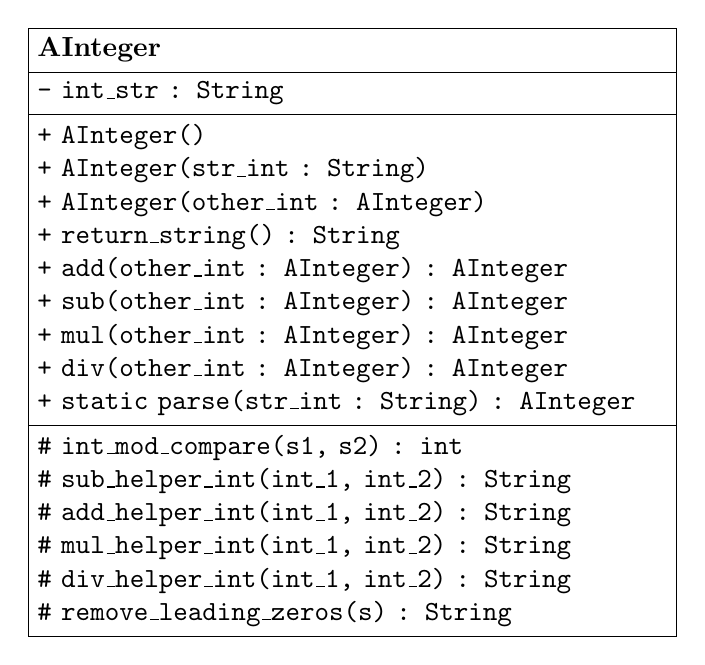
\begin{tikzpicture}
  \node[rectangle split, rectangle split parts=4, draw, text width=8cm, align=left] (AInteger) 
    {
      \textbf{AInteger}
      \nodepart{second}
      \texttt{- int\_str : String}
      \nodepart{third}
      \texttt{+ AInteger()}\\
      \texttt{+ AInteger(str\_int : String)}\\
      \texttt{+ AInteger(other\_int : AInteger)}\\
      \texttt{+ return\_string() : String}\\
      \texttt{+ add(other\_int : AInteger) : AInteger}\\
      \texttt{+ sub(other\_int : AInteger) : AInteger}\\
      \texttt{+ mul(other\_int : AInteger) : AInteger}\\
      \texttt{+ div(other\_int : AInteger) : AInteger}\\
      \texttt{+ static parse(str\_int : String) : AInteger}\\[0.5em]
      \nodepart{fourth}
      \texttt{\# int\_mod\_compare(s1, s2) : int}\\
      \texttt{\# sub\_helper\_int(int\_1, int\_2) : String}\\
      \texttt{\# add\_helper\_int(int\_1, int\_2) : String}\\
      \texttt{\# mul\_helper\_int(int\_1, int\_2) : String}\\
      \texttt{\# div\_helper\_int(int\_1, int\_2) : String}\\
      \texttt{\# remove\_leading\_zeros(s) : String}
    };
\end{tikzpicture}
\subsection{AFloat.java}
\subsubsection{Addition}
\begin{itemize}
    \item Both floating-point numbers were converted to integers by removing the decimal point and padding with appropriate zeroes. The resulting integers were then added using the method defined in AInteger.java.
    \item The sign of the result was determined and applied in the same manner as in AInteger.java.
    \item StringBuilder was used for efficient string manipulation (e.g., removing and re-inserting the decimal point), minimizing the creation of intermediate string objects.
\end{itemize}
\subsubsection{Subtraction}
\begin{itemize}
    \item Similar to addition, both floats were treated as integers by removing the decimal point and padding with zeroes. The subtraction method from AInteger.java was then used.
    \item Final sign determination and immutability were handled consistently with the addition method.
\end{itemize}
\subsubsection{Multiplication}
\begin{itemize}
    \item Decimal points were removed from both operands, converting them into integers. Multiplication was then performed using the method in AInteger.java.
    \item The operand with fewer digits after the decimal point was padded with zeroes to match the other. This facilitated accurate decimal placement in the final result.
\end{itemize}
\subsubsection{Division}
\begin{itemize}
    \item Both floats were converted into integers by removing the decimal points and padding with zeroes. Division was then performed using the method from AInteger.java.
    \item Padding ensured equal decimal precision for easier placement of the decimal point in the quotient.
    \item A mechanism was implemented to handle 30-decimal precision in the decimal portion of the result.
\end{itemize}
\subsubsection{UML diagram for AFloat.class}
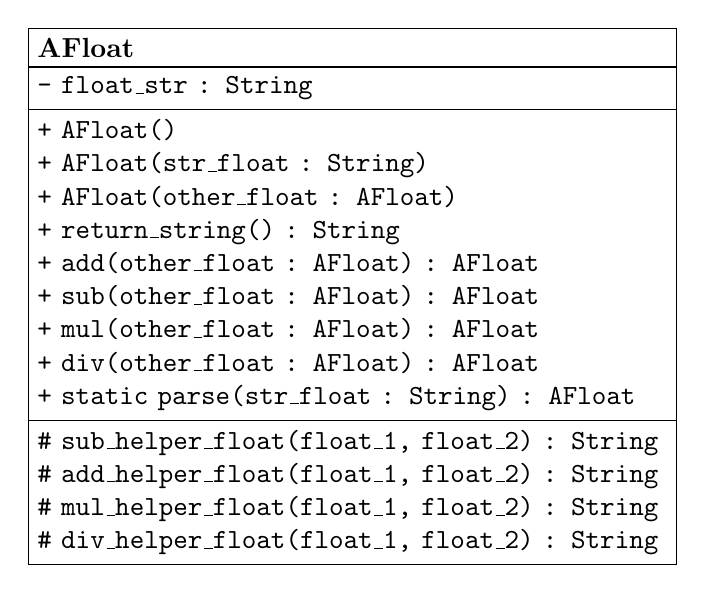
\begin{tikzpicture}
  \node[rectangle split, rectangle split parts=4, draw, text width=8cm, align=left] (AInteger) 
    {
      \textbf{AFloat}
      \nodepart{second}
      \texttt{- float\_str : String}
      \nodepart{third}
      \texttt{+ AFloat()}\\
      \texttt{+ AFloat(str\_float : String)}\\
      \texttt{+ AFloat(other\_float : AFloat)}\\
      \texttt{+ return\_string() : String}\\
      \texttt{+ add(other\_float : AFloat) : AFloat}\\
      \texttt{+ sub(other\_float : AFloat) : AFloat}\\
      \texttt{+ mul(other\_float : AFloat) : AFloat}\\
      \texttt{+ div(other\_float : AFloat) : AFloat}\\
      \texttt{+ static parse(str\_float : String) : AFloat}\\[0.5em]
      \nodepart{fourth}
      \texttt{\# sub\_helper\_float(float\_1, float\_2) : String}\\
      \texttt{\# add\_helper\_float(float\_1, float\_2) : String}\\
      \texttt{\# mul\_helper\_float(float\_1, float\_2) : String}\\
      \texttt{\# div\_helper\_float(float\_1, float\_2) : String}\\
    };
\end{tikzpicture}
\subsection{MyInfArith.py}
\begin{itemize}
    \item The argparse library was utilized to handle command-line arguments for the Python script. By leveraging the choices parameter, it significantly reduces the likelihood of invalid inputs and associated errors.
    \item JPype was employed to seamlessly import and interact with Java classes within the Python environment, enabling cross-language integration.
    \item While argparse's choices feature prevents many common input errors, additional validation was implemented to handle edge cases-such as verifying whether input strings can be correctly parsed as integers or floats.
\end{itemize}
\section{UML diagram}
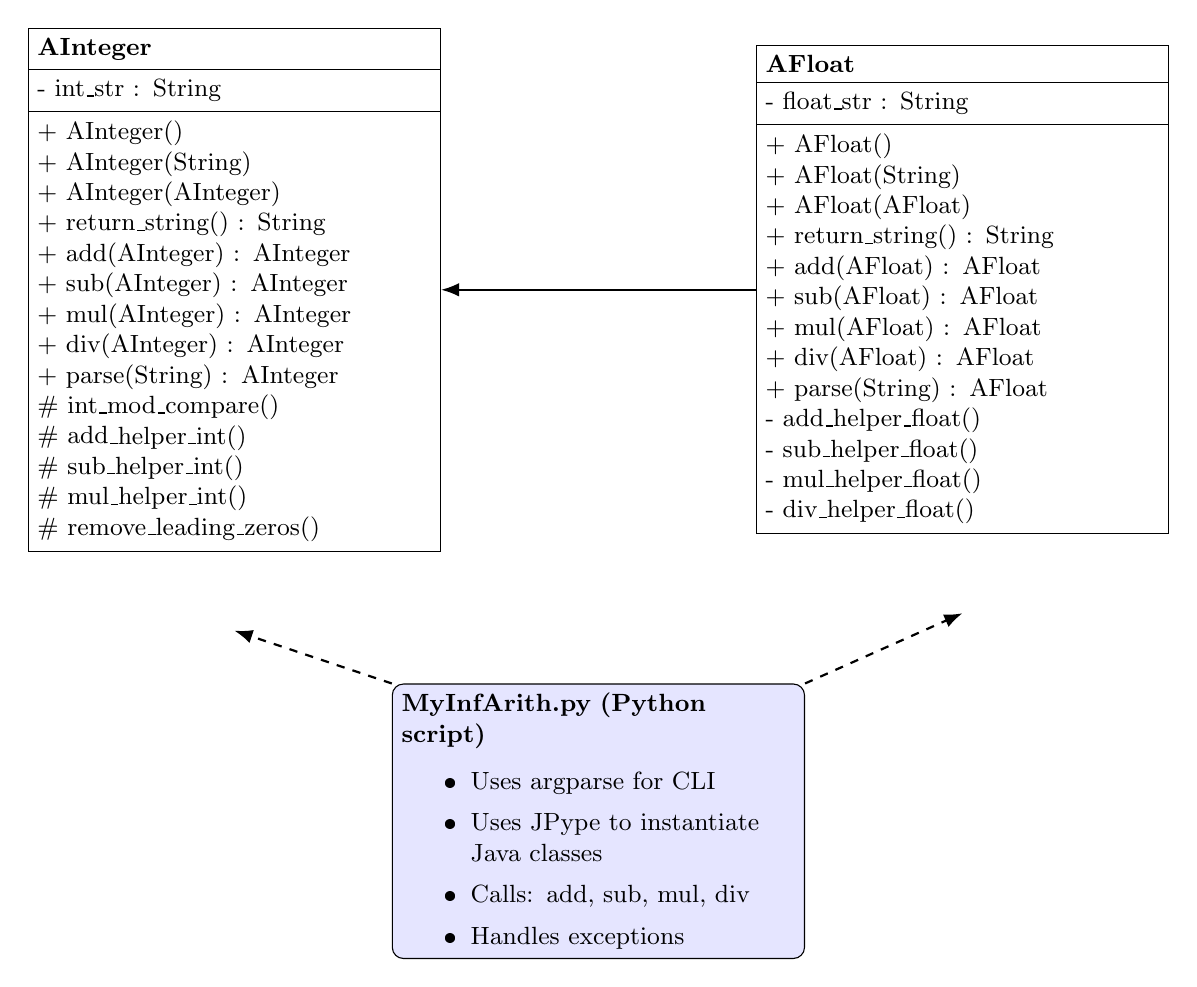
\begin{tikzpicture}[
    class/.style={
        rectangle split,
        rectangle split parts=3,
        draw,
        rectangle split part align={center,left,left},
        text width=5cm,
        minimum height=2cm,
        font=\small
    },
    note/.style={
        rectangle,
        draw,
        fill=blue!10,
        text width=5cm,
        rounded corners,
        font=\small
    },
    inherit/.style={-Latex, thick},
    uses/.style={dashed, -Latex, thick}
]

% AInteger class
\node[class] (AInteger) {
    \textbf{AInteger}
    \nodepart{second}
    - int\_str : String
    \nodepart{third}
    + AInteger()\\
    + AInteger(String)\\
    + AInteger(AInteger)\\
    + return\_string() : String\\
    + add(AInteger) : AInteger\\
    + sub(AInteger) : AInteger\\
    + mul(AInteger) : AInteger\\
    + div(AInteger) : AInteger\\
    + parse(String) : AInteger\\
    \# int\_mod\_compare()\\
    \# add\_helper\_int()\\
    \# sub\_helper\_int()\\
    \# mul\_helper\_int()\\
    \# remove\_leading\_zeros()
};

% AFloat class
\node[class, right=4cm of AInteger] (AFloat) {
    \textbf{AFloat}
    \nodepart{second}
    - float\_str : String
    \nodepart{third}
    + AFloat()\\
    + AFloat(String)\\
    + AFloat(AFloat)\\
    + return\_string() : String\\
    + add(AFloat) : AFloat\\
    + sub(AFloat) : AFloat\\
    + mul(AFloat) : AFloat\\
    + div(AFloat) : AFloat\\
    + parse(String) : AFloat\\
    - add\_helper\_float()\\
    - sub\_helper\_float()\\
    - mul\_helper\_float()\\
    - div\_helper\_float()
};

% Inheritance arrow
\draw[inherit] (AFloat.west) -- ++(-1,0) |- (AInteger.east);

% MyInfArith.py note
\node[note, below=5cm of $(AInteger)!0.5!(AFloat)$] (MyInfArith) {
    \textbf{MyInfArith.py (Python script)}\\
    \begin{itemize}
        \item Uses argparse for CLI
        \item Uses JPype to instantiate Java classes
        \item Calls: add, sub, mul, div
        \item Handles exceptions
    \end{itemize}
};

% Usage arrows
\draw[uses] (MyInfArith.north west) -- ([yshift=-1cm]AInteger.south);
\draw[uses] (MyInfArith.north east) -- ([yshift=-1cm]AFloat.south);

\end{tikzpicture}
\section{README: Usage of the library}
\subsection{Overview}
This project presents a custom Java library designed for arbitrary-length and high precision floating-point arithmetic, built from scratch without relying the Java's built-in classes.
\subsection{Python CLI}
Make sure that the current directory is the project directory
\begin{tcolorbox}[colback=black, colframe=white!25!black, coltext=white, title=terminal]
\texttt{cd projectdirectory}
\end{tcolorbox}
Run the build file using Python CLI
\begin{tcolorbox}[colback=black, colframe=white!25!black, coltext=white, title=terminal]
\texttt{python MyInfArith int add 45 3}
\end{tcolorbox}
The output is as follows
\begin{tcolorbox}[colback=black, colframe=white!25!black, coltext=white, title=terminal]
\texttt{48}
\end{tcolorbox}

\subsection{Running through docker docs}
Steps for using dockerhub:
\begin{itemize}
    \item Use the dockerfile in the repo
    \begin{tcolorbox}[colback=black, colframe=white!25!black, coltext=white, title=terminal]
\texttt{docker build -t imagename .}
\end{tcolorbox}
This opens a shell of the docker container
\begin{tcolorbox}[colback=black, colframe=white!25!black, coltext=white, title=terminal]
\texttt{docker run -it imagename bash}
\end{tcolorbox}
\item To push
\begin{tcolorbox}[colback=black, colframe=white!25!black, coltext=white, title=terminal]
\texttt{docker tag imagename username/officialimagename:tag}
\end{tcolorbox}
\begin{tcolorbox}[colback=black, colframe=white!25!black, coltext=white, title=terminal]
\texttt{docker push username/officialimagename:tag}
\end{tcolorbox}
\end{itemize}
\section{Git Commits}
\begin{tcolorbox}[colback=black, colframe=white!25!black, coltext=white, title=terminal]
\texttt{* 1aa3857 (HEAD -> master, origin/master) Stop tracking p.py\\
$*$ f355022 Stop tracking p.py\\
$*$ f54f243 Built a docker container\\
$*$ 24dabab added ant and README.md\\
$*$   417fb1d Merge remote-tracking branch 'origin/master' merging git\\
|\ \\
| * 4feb80a Create README.md\\
$*$ | c71b5b2 added ant file\\
|/\\
$*$ eea42ab Completed the automation\\
$*$ 20e70e1 Modified AFloat to handle int operands\\
$*$ 5546bc3 Appropriate operations done\\
$*$ df1f2e6 Added required arguments and checking the validity of inputs\\
$*$ 6e76bbb Added the division by zero exception in AFloat class\\
$*$ 294e23c Tidied up the code a bit\\
$*$ e799b10 Deleting the java automation files\\
$*$ 6162083 Delete directory My\_Project\\
$*$ 2ab8b1d Python automation file added\\
$*$ eaa5ed4 Comments added to AFloat.java, and its add and sub methods were changed\\
$*$ 125014e Comments added to AInteger.java\\
$*$ e0db5c4 Float division method added\\
$*$ 793ad72 Float multiplication method added\\
$*$ fa0ae7e Float addition method added\\
$*$ f7c4bc7 Float subtraction method added\\}
\end{tcolorbox}
\section{Verification}
\begin{itemize}
    \item Manual testing of corner cases such as large integers beyond standard int range.
    \item Comparison with Java's BigInteger and BigDeciaml for validation.
\end{itemize}
\section{Key Learnings}
\begin{itemize}
    \item Understanding of argparse library and its benefits , and Jpyp library used to bridge Python and Java.
    \item Working with \textbf{ant} automation system
    \item Using \textbf{Docker}
    \item Generating UML diagrams in LaTex.
    \item Basic idea of Markdown language.
\end{itemize}
\section{Possible improvements}
\begin{itemize}
    \item Instead of fixing the precision to 30 decimals, taking an input for precision from the user would have made it more flexible.
\end{itemize}

\end{document}
